\chapter{Grundlagen} 
\label{ch:grundlagen}
In diesem Kapitel möchte ich einige Grundlagen für die weiteren Kapitel dieser Arbeit legen. Zunächst erläutere ich den Aufbau eines neuronalen Netzes im allgemeinen, die Bedeutung von rekurrenten neuronalen Netzen (RNN), zeige am Bouncing Ball Szenario das Vanishing Gradient Problem auf und mache so die Notwendigkeit der LSTM-Technik deutlich.
\section{Neuronale Netze}
Als neuronales Netz bezeichnet man eine verwobene Struktur zwischen vielen einzelnen Zellen von meistens gleichem - aber keineswegs darauf beschr\"anktem - Aufbau, den sogenannten Neuronen. Eine solche Zelle hat immer die Eigenschaft, dass sie Signale von anderen Zellen empfängt, diese gewichtet aufakkumuliert und abhängig von einer internen Aktivierungsfunktion ein entsprechendes Signal an andere Zellen weitergibt, die damit ihrerseits diesselbe Prozedur durchlaufen. Ein neuronales Netz im Gehirn einer Ameise hat ca. 250.000 Neuronen, ein menschliches 86 Milliarden \cite{bib:number} und wir haben lediglich eine wage Vorstellung, wozu diese imstande sind. In der Informatik werden solche Strukturen als künstliche neuronale Netze nachgebildet und je nach Problemstellung abgewandelt. Zur Vereinfachung meinen wir ab sofort, sofern nicht explizit anders angegeben, mit neuronalen Netzen künstliche neuronale Netze.
\begin{figure}
	\centering
	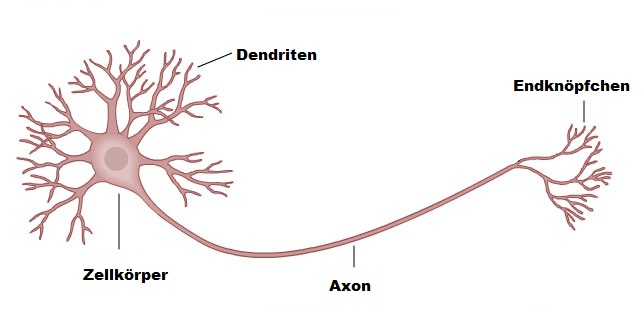
\includegraphics[width=0.7\textwidth, height=130px]{pics/neuron.jpg}	
	\caption{Schematische Darstellung eines biologischen Neuron \cite{bib:neuron}}
	\label{img:neuron}
\end{figure}
\begin{figure}
	\centering
	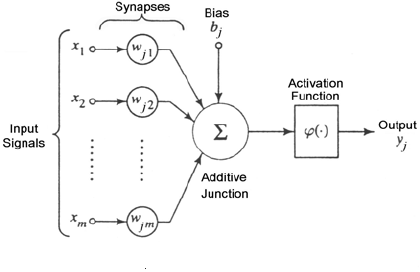
\includegraphics[width=0.7\textwidth, height=130px]{pics/aneuron.png}	
	\caption{Schematische Darstellung einer Möglichkeit, ein künstliches Neuron zu simulieren \cite{bib:aneuron}}
	\label{img:aneuron}
\end{figure}
\begin{figure}
	\centering
	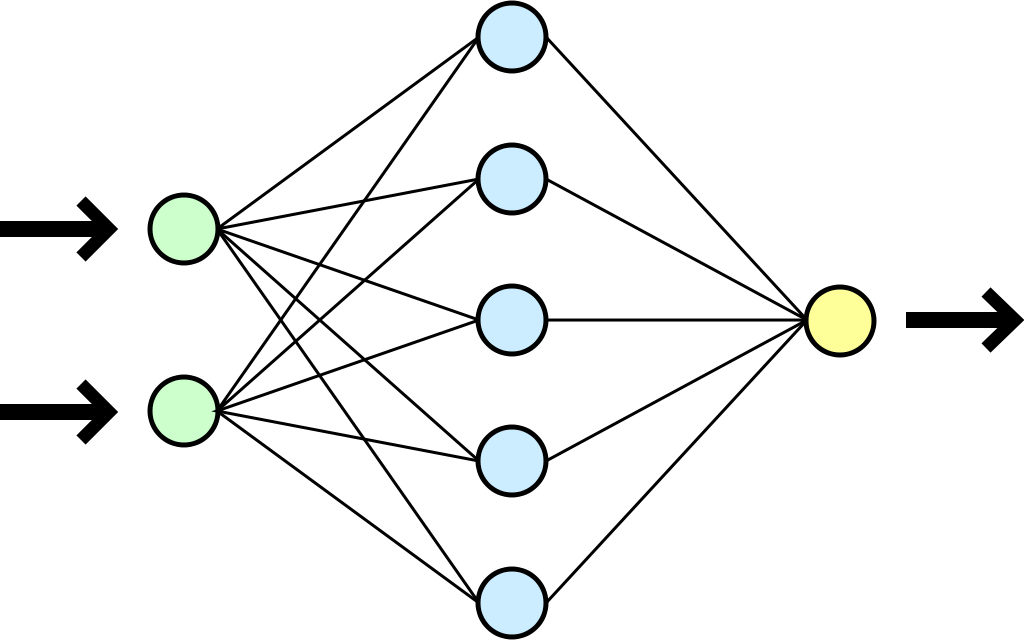
\includegraphics[width=0.7\textwidth, height=130px]{pics/MLP.png}	
	\caption{Ein Multilayer Perceptron mit 2 Inputneuronen(grün), einem Hidden Layer mit 5 Neuronen(blau) und einem einzelnen Outputneuron(gelb).   \cite{bib:mlp}}
	\label{img:mlp}
\end{figure}
Es gibt viele verschiedene Arten von neuronalen Netzen, die einfachste von Ihnen ist das Multilayer Perceptron (MLP). Die Zellen werden zu mehreren Ebenen(Layer) zusammengefügt. Erst das Inputlayer, in das die Daten hineingegeben werden, dann die versteckten Layer, versteckt weil hier wie in einer Blackbox die Berechnungen passieren und dann an das Outputlayer weiterleitet, aus welchem das Ergebnis des Netzes kommt.Es gibt eine geordnete Datenflussrichtung, eine Zelle erhält ihren Input von jeder Zelle der vorigenen Ebene und gibt ihren Output entsprechend an jede Zelle der folgenden Ebene weiter, Feedforward genannt. Ein solches Netz sieht man in Abbildung \ref{img:mlp}.  
\begin{gather}
x_{j} = \varphi_{h}(net_{h}) = \varphi_{h}(\sum_{i=1}^{n} x_{i}w_{ij}) 
\label{eq:act}
\end{gather}
In jeder Zelle \(j\) werden die Inputsignale \(x_{i}\), also die Aktivierungen der vorigen Zellen mit Index \(i\) unterschiedlich gewichtet \(w_{ij}\) aufsummiert \(net_{h}\) (Abbildung \ref{img:aneuron}).  Eben diese Gewichte sind der Kern des maschinellen Lernens, da bei einmal geschickt gefundenen Gewichten, komplexe Aufgabenstellungen und Probleme mit (vergleichsweise) wenig Rechen- sowie Programmieraufwand gelößt werden können. Im Wesentlichen versucht ein MLP immer eine Funktion zu berechnen welches einen Inputvektor der Größe \(n\) auf einen Outputvektor der Größe \(m\) abbildet.
\begin{gather*}
f_{MLP}: R^n \to R^m 
\end{gather*}
Ein Beispiel für eine solche Funktion wäre für ein gegebenes Bild zu entscheiden, ob darauf ein Gesicht zu erkennen ist. Die Länge des Inputs wäre hier z.B. mehrere Millionen, einfach die Pixelwerte, als Output wäre hier nur eine Zahl, nämlich ob ein Gesicht zu sehen ist oder nicht. Der Output \(y\) des Netzes ist also abhängig vom Input \(x\), aber auch von den Gewichten \(w\).
Die Gewichte werden entweder mit Hilfe von Trainingsdaten, bestehend aus Inputdaten und entsprechenden Outputdaten, also den zugehören Lösungen, oder mit einer zu erlenenden Zielfunktion, die einem aus gegebenen Inputdaten die gewünschten Lösungen liefert, über mehrere Trainingsläufe (Epochen) justiert. Fügt man in die Inputebene entsprechende Inputdaten \(x\) ein, berechnet die Aktivierungen aller Zellen, vergleicht die Aktivierungen \(y\) des Outputlayers des Netzes mit den gegebenen Lösungen \(z\) und erhält eine Fehlerabweichung \( E(z,y)\): 
\begin{equation}
E(z,y) =_{def} \dfrac{1}{2} \sum_{i=1}^{m}(z_{i}-y_{i})^{2}
	\label{eq:err}
\end{equation}
Die Herausforderung ist es nun, diejenigen Gewichte \(w\) zu finden, für die die Fehlerabweichung über alle Trainingsdaten minimal ist.
\begin{equation}
arg_{w} min( \sum_{(x,z)\in trainset} E(z,f_{MLP}(w,x)))
\label{eq:err}
\end{equation}
Bei der Anpassung der Gewichte der versteckten Zellen hat man aber das Problem, das man keinen direkten Fehler für sie kennt, da man nur für die Outputschicht den gewünschten Output hat und so einen Fehler ermitteln kann. Als Lösung ist hier der Backpropagation-Algorithmus geläufig. Dieser besteht aus 3 Schritten, die entweder solang durchlaufen werden bis der Fehler einen festgesetzten Schwellenwert(Threshold) unterschreitet, oder eine vorgegebene Anzahl an Epochen durchlaufen wurde. 
\begin{description}	\item[Feedforward]\hfill \\
	Das Inputlayer wird mit der Eingabe des jeweiligen Testsatzes befüllt und die Aktivierungen vorwärts Layer für Layer, Zelle für Zelle berechnet.  
	\item[Backward-Pass]\hfill \\ 
	Das Ergebnis am Outputlayer wird mit der gewünschten Lösung des Testsatzes verglichen und der Fehler berechnet. Diese werden entsprechend gewichtet die unteren Layer rückwärts Zelle für Zelle rückpropagiert. Oft werden hier statt dem tatsächlichen Fehler direkt der Gradient bzw. ein Zwischenwert für dessen Berechnung propagiert\ref{eq:bp}.
	\item[Anpassen der Gewichte]\hfill \\ Dies ist der wichtige Schritt, hier werden nun Zelle für Zelle die Gewichte entsprechend des Gradienten angepasst. Mit den neuen Gewichten ist in der Regel der Output des Netzes genauer, der Fehler also geringer und der Algorithmus lässt die Fehlerfunktion im Idealfall gegen 0 konvergieren.\cite{bib:nn}
\end{description}
Die Gewichte werden anhand eines absteigenden Gradienten der Fehlerfunktion, abgeleitet nach den Gewichten \(w_{ij}\), aktuallisiert.  Hierzu werden die \(\delta\), die aufsummierten Fehler für jede Zelle wie folgt berechnet: 
\begin{gather}
\delta_{k} = \varphi_{k}'(net_{k})(x_{k}-z_{k}) \\
\delta_{h} = \varphi_{h}'(net_{h})\sum_{k\in K}w_{hk}\delta_{k} 
\label{eq:err}
\end{gather}

Wobei erst nach der oberen Gleichung für die Outputlayer die \(\delta_{k}\) gebildet und in die jeweils unteren Layer nach der unteren Gleichung beim bilden der \(\delta_{h}\) gewichtet aufsummiert werden (Backpropagation). \textit{K} sind hier die Neuronen aus dem jeweils oberen Layer. Die Formel für das Gewichtsupdate mit einer Lernrate \(\eta\) lautet dann:
\begin{gather}	
	\Delta w_{ij} =_{def}  -\eta \frac{\partial E}{\partial w_{ij}} = -\eta x_{i}\delta_{j}  
\end{gather} 
Formel zur Berechnung der Gewichtupdates aus dem Gradienten der Fehlerfunktion \cite{bib:bp}\\
Es gibt nun noch verschiedene Techniken um das Ergebnis weiter zu verbessern und das lernen noch schneller und stabiler zu machen, an dieser Stelle wollen wir unser Augenmerk aber in eine andere Richtung lenken. 
\section{Rekurrente Neuronale Netze}

Neuronale Netzwerke haben einen für einen 1-Dimensionalen Inputvektor einen eindeutig zu berechnenden 1-Dimensionalen Outputvektor und für die meisten Problemstellungen ist auch genau diese Kompetenz gefordert. Es gibt aber auch Probleme, bei denen der Output nicht nur von diesem, sondern auch von allen beziehungsweise einigen vorigen Inputs und Zuständen abhängt. Ein anschauliches Beispiel wäre hier die Klassifizierung von Videoausschnitten, wo die Bedeutung eines einzelnen Frames vom Kontext der vorigen Frames abhängt, hingegen ein einfacheres Beispiel wäre das in dieser Arbeit betrachtete Bouncing Ball Szenario. Befindet sich ein Ball im Punkt \(p_{1}=(0/0)\) und der nächste Ort \(p_{2}\) soll vorhergesagt werden, ist es natürlich entscheidend ob der Ball sich zuvor beispielsweise im Punkt \(p_{0}=(0.1/0,1)\) oder im Punkt \(p_{0}=(-0.1/-0.1)\) befand. Hierzu werden den Zellen aus dem verstecktem Layer des neuronalen Netzes rekurrente (lat. recurrere:zurücklaufen) Verbindungen hinzugefügt.
\begin{figure}
	\centering
	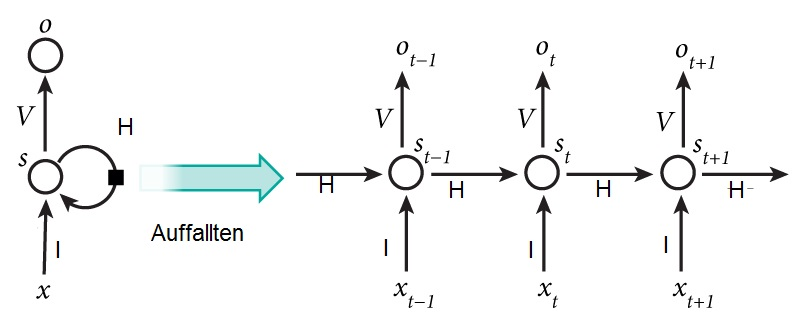
\includegraphics[width=0.7\textwidth, height=130px]{pics/rnn.jpg}	
	\caption{Um Backpropagation für ein rekurrentes Netz zu benutzen, muss man es durch die Zeit auffallten. \cite{bib:rnn}}
	\label{img:rnn}
\end{figure}
Eine Zelle \textit{h} bekommt nun im Zeitpunkt \textit{t} seinen Input immernoch von allen Zellen des unteren Layers \textit{I}, zusätzlich nimmt sie aber auch noch als Input den Output aller Zellen desselben Layers, aber aus dem vorigen Zeitschritt \textit{H'}, die Formel für die Aktivierung lautet also: 
\begin{gather}
x^{t}_{h}=\varphi_{h}(net_{h}^{t})=\varphi_{h}(\sum_{i \in I}w_{ih}x^{t}_{i}+\sum_{i \in H'}w_{h'h}x^{t-1}_{h'})
\end{gather}

Da diese neuen rekurrenten Inputs auch wieder gewichtet verarbeitet werden, müssen diese erst noch geschickt gefunden werden. Dies macht man mit Backpropagation durch die Zeit (BPTT). Dies passiert analog zur Backpropagation im MLP, jedoch werden die einzelnen Zeitschritte aufgeklappt (Abbildung \ref{img:rnn}). Die Backpropagation through time berechnet sich also wiefolgt:
\begin{gather}
	\delta_{k}^{t} = \varphi_{k}'(net_{k}^{t})(x_{k}^{t}-z^{t}_{k}) \\
	\delta_{h}^{t} = \varphi_{h}'(net_{h}^{t})(\sum_{k \in K}w_{hk}\delta^{t}_{k}+\sum_{h' \in H'}w_{hh'}\delta^{t+1}_{h'})
\end{gather}

Wobei hier die obere Formel wieder für jedes Neuron des Outputlayers und die untere für die Hiddenlayer. Für das Gewichtsupdate werden die Deltas noch über den betrachteten Zeitraum aufsummiert und analog zum Multilayer Perzeptron berechnet. Den Backpropagation Algorithmus anwenden um das Netz zu trainieren und passende Gewichte, auch für die rekurrenten Verbindungen zu erhalten. Nun hat man ein Neuronales Netz mit einer Art Kurzzeitgedächtnis, welches beim Auswerten des Inputs die Nahe Vergangenheit mit in Betracht zieht. Hat es in der Anwendung aber tiefere Abhängigkeiten, wo ein vergangener Input einen Einfluss auf die fernere Zukunft hat, hat auch das RNN noch Schwierigkeiten: 
\section{Das Vanishing Gradient Problem}
\begin{figure}
	\centering
	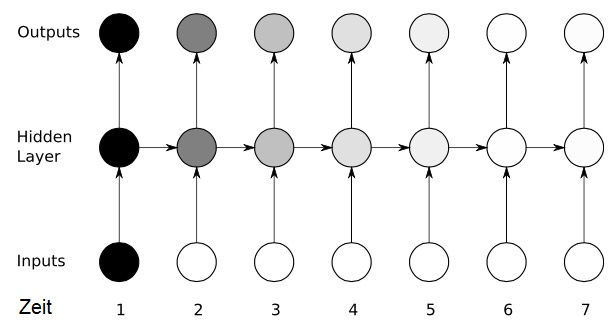
\includegraphics[width=0.7\textwidth, height=130px]{pics/vgp.jpg}	
	\caption{Das Problem vom verschwindendem Gradienten in einem rekurrenten Netz. Ein Fehler im Zeitschritt 1 erzeugt einen Gradienten, der aber auf die folgenden Zeitschritte immer weniger Einfluss hat.\cite{bib:vgp}}
	\label{img:vgp}
\end{figure}
Wir haben gesehen wie beim Training eines rekurrenten Netzes über die Bildung des Gradienten geschickt Gewichte gefunden werden, die Probleme lösen können bei denen Abhängigkeiten über die Zeit auftreten. Erstrecken sich diese Abhängigkeiten aber über zu große Zeitraume, tritt das Problem vom verschwindendem Gradienten auf. Mit den üblichen Aktivierungsfunktionen wie z.B der \textit{tanh}-Funktion treten Gradienten mit Betrag \(\leq\) 1 auf, bei der \textit{sigmoid}-Funktion sogar \(\leq 0.25\), die bei Backpropagation per Kettenregel miteinander multipliziert werden. Wird nun im Frontlayer ein Gradient berechnet, werden für \textit{n}-Layer im Netz, also auch für ein rekurrentes Netz das um \textit{n} Zeitschritte aufgefalltet wird, \textit{n} dieser kleinen Zahlen miteinander multipliziert, wodurch der Gradient exponentiell schnell sinkt. Hat man hingegen eine Aktivierungsfunktionen mit Gradienten Betrag \(\geq 1\), wächst der Gradient exponentiell schnell, das Exploding Gradient Problem.

Es bleibt aber zu erwähnen, dass dieses Problem nur beim automatisierten Training eines rekurrenten Netzes auftritt. Wenn man die Gewichte vorgibt und Aktivierungsfunktionen geschickt wählt, kann ein rekurrentes Netz Zellen als Speicherzellen verwenden, z.B. indem es immer den Wert den es im letzten Zeitschritt als Output hatte als Input nimmt, indem es nur dem rekurrenten Gewicht zur eigenen Zelle den Wert 1 gibt. Sinnvoll ist die Speicherzelle natürlich nur, wenn sie auch befüllt werden kann, durch sogenannte Gate-Zellen. Eine Inputgate-zelle, welches reguliert ob, und mit was die Speicherzelle befüllt wird, eine Forgetgate-Zelle, welche die Speicherzelle wieder leeren kann und auch eine Outputgate-Zelle die steuert ob die Speicherzelle ihren Inhalt ausgibt, sind Strukturen die mit rekurrenten Neuronalen Netzen möglich sind und im kleinen Maß auch einfach zu erzeugen, wenn man die Gewichte manuell auswählen würde. Praktisch ist ein Neuronales Netz aber natürlich nur, wenn die Gewichte automatisch durch geschicktes Training gefunden werden, dass solche Strukturen aber zufällig erzeugt werden ist aber mit den bisher bekannten Trainingsmethoden quasi unmöglich. Wenn man jedoch eine geschickte Struktur fest vorgibt, funktioniert das Training und das Vanishing Gradient Problem wird überwunden. Eine mögliche solche Struktur sind die LSTM Zellen. 
\section{LSTM}
\begin{figure}
	\centering
	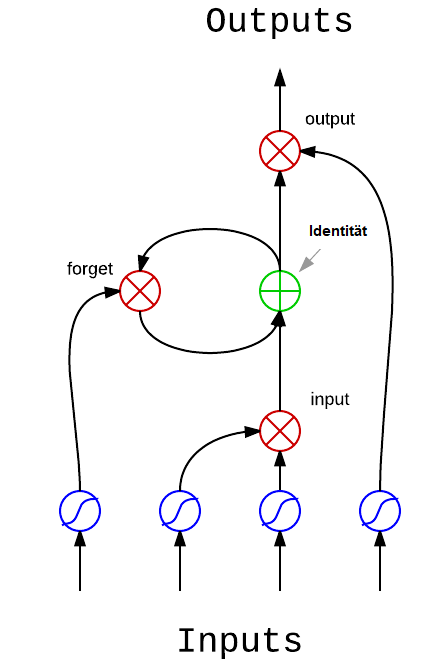
\includegraphics[width=0.5\textwidth, height=300px]{pics/lstm.png}	
	\caption{Ein Aufbau einer LSTM-Speicherzelle. 4 rekurrente Neuronen (blau), die die 3 multiplikativen Gates lenken (rot), die das Verhalten der Speicherzelle steuern.    \cite{bib:lstm}}
	\label{img:lstm}
\end{figure}
LSTM steht für long short-term memory, zu deutsch, langes Kurzzeitsgedächtnis, ist eine Struktur die man in rekurrente neuronale Netze einbaut um Speicherzellen zu haben, die Werte stabil über beliebig viele Zeitschritte speichern können. Üblich ist hierfür ein Aufbau wie in Abbildung \ref{img:lstm}. 4 normale rekurrente Neuronen, die als Input also Aktivierungen des darunterliegenden Layers sowie die desselben Layers, aber des vorrigen Zeitschritts, bekommen und daraus ihre eigene Aktivierung berechnen, steuern das Verhalten der Speicherzelle. Eines steuert das Forget-Gate, also ob die Speicherzelle ihren gespeicherten Wert behalten soll. Im Normalzustand hat das Forgetgate den Wert 1, sodass der gespeicherte Wert multipliziert mit 1 der Wert selbst bleibt. Soll ein Wert vergessen, bzw. nichts gespeichert werden, muss das Forgetgate den Wert 0 annehmen. 2 Zellen steuern das Inputgate, eine gibt den Wert an, welcher gespeichert werden soll und die andere steuert mit einem Wert zwischen 0 und 1, ob die Zelle einen neuen Wert speichert. Es gibt Varianten, wo das Input- und das Forgetgate gekoppelt sind, sodass immer wenn ein neuer Wert gespeichert werden soll der alte gelöscht wird und umgekehrt, ist dies nicht der Fall, wird das Ergebnis des Inputgates auf den bisher gespeicherten Wert aufaddiert. Die 4. Zelle steuert das Outputgate, interaggiert also nicht mit dem Wert der Speicherzelle selbst, aber regelt ob das gespeicherte ausgegeben wird oder nicht. \cite{bib:lstm2}

In Abbildung \ref{img:lstm2} sieht man, wie der Inhalt der Speicherzellen sauber durch die Gates gelenkt werden können. Das funktioniert im Forwardpass, aber auch genauso beim Training im Backwardpass mit dem Gradienten, da der Inhalt der Zelle per Identitätsfunktion durch die Zeit auf sich selbst abgebildet wird, und da der Gradient der Identität den Betrag \( = 1 \) hat, geht jetzt auch nichts mehr verloren. \cite{bib:lstm}. LSTM Netze werden wie rekurrente Netze trainiert, mit Backpropagation through time.
\begin{figure}
	\centering
	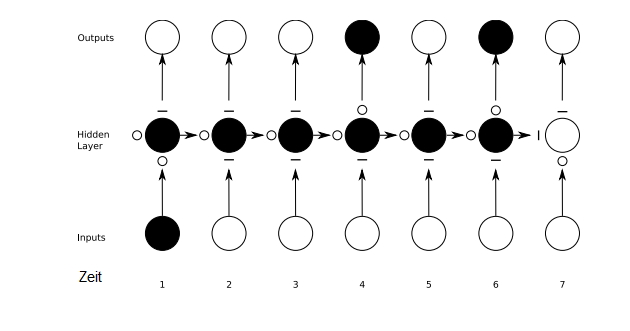
\includegraphics[width=0.7\textwidth, height=130px]{pics/lstm2.png}	
	\caption{Der Inhalt der Zelle wird durch die verschiedenen Zeitschritte durch die Gates gelenkt. Kreis bedeutet offenes Gate, ein Querstrich stellt ein geschlossenes Gate dar.    \cite{bib:lstm}}
	\label{img:lstm2}
\end{figure}

LSTM wird in aktuellen Produkten von bedeutenden Technologie Firmen wie zum Beispiel Apple\cite{bib:apple}, Amazon\cite{bib:amazon} und Google als Kernkomponente verwendet, von Google zum Beispiel für die Spracherkennung für den Smartphoneassistenten Allo\cite{bib:allo}. 

Nun wollen wir in dieser Arbeit untersuchen, wie das LSTM in seinen Zellen mit Events umgeht. Für die Unterteilung durch Events gibt es aus der Psyhologie bereits einen Ansatz, die Event Segmantation Theory (EST).

\section{Event Segmentation Theory}
Ein Weg etwas zu verstehen, ist es in kleinere Teile zu Unterteilen. Nach der Event Segmentation Theory (Zacks et al. 2007) ist das Unterteilen von kontinuirlicher Aktivität durch bedeutungsvolle Ereignisse eine Kernkompnente der Wahrnemung. \cite{bib:est} Dies ist sowohl ein Top-Down also auch ein Bottom-Up Vorgang, also sowohl das Wissen über die Pläne des beobachteten Akteurs als auch der direkte sensorische Input haben Einfluss auf diese Unterteilung.\cite{bib:est1} Die Planung zum erreichen eines Ziels ist in Events unterteilt, z.B. wenn man jemandem zuschaut sein Zelt aufzubauen, erwartet man, wenn man den Vorgang kennt, dass dieser erst das Zelt aus der Verpackung holt, das Zelt ausbreitet, die Stangen zusammensteckt, usw.. Diese Unterteilung ist für uns ganz natürlich und dazu macht es keinen Unterschied, ob man sich zum Zusammenstecken der Stangen z.B. auf den Boden setzt, auch wenn das physich ein ganz anderer Vorgang ist. Die Bottom-Up Seite von EST ist greift auf ein Model zurück, bei dem unser Gehirn ständig Vorhersagen über die Umwelt macht und resultierene entdeckte Fehler verarbeitet \cite{bib:est1}. Befindet sich der beobachtete Akteur in einem Event, werden sich dessen folgenden Bewegungen und Aktionen stetig an seine vergangenen Aktionen anschließen. Hat man hingegen eine hohe Unsicherheit in der Vorhersage der nächsten Aktionen, wird eine Eventunterteilung vorgenommen. Am Beispiel: Ist jemand gerade beschäftigt mit dem zusammenstecken der Zeltstangen, wird er das erfahrungsgemäß auch weitertun, ist er damit aber fertig, ist unklar ob er z.B. erst das Vorzelt aufbaut, uns als Beobachter um Hilfe bittet oder sich erstmal einen Kaffee holt. 
Entgegen dem alltäglichen Sprachgebrauch meint EST mit Ereignissen immer ganze Vorgänge, also z.B. das zusammenstecken der Zeltstangen, nicht aber das Beginnen oder das Fertigwerden, diese werden als Ereignisgrenzen bezeichnet. Ereignisse sind verschieden Granuliert und hierarchisch, so ist z.B. das zusammenstecken der Zeltstangen teil des Ereignisses des Zeltaufbauens welches wiederrum teil des Ereignisses Campingurlaub ist.

In Abbildung \ref{img:est} sieht man, wie eine Unterteilung nach Bedeutung dem Verstehen hilft. EST sieht seine Gültigkeit sowohl beim beurteilen und vorhersagen der Aktionen anderer, als auch beim durchführen und planen der eigenen.


\begin{figure}
	\centering
	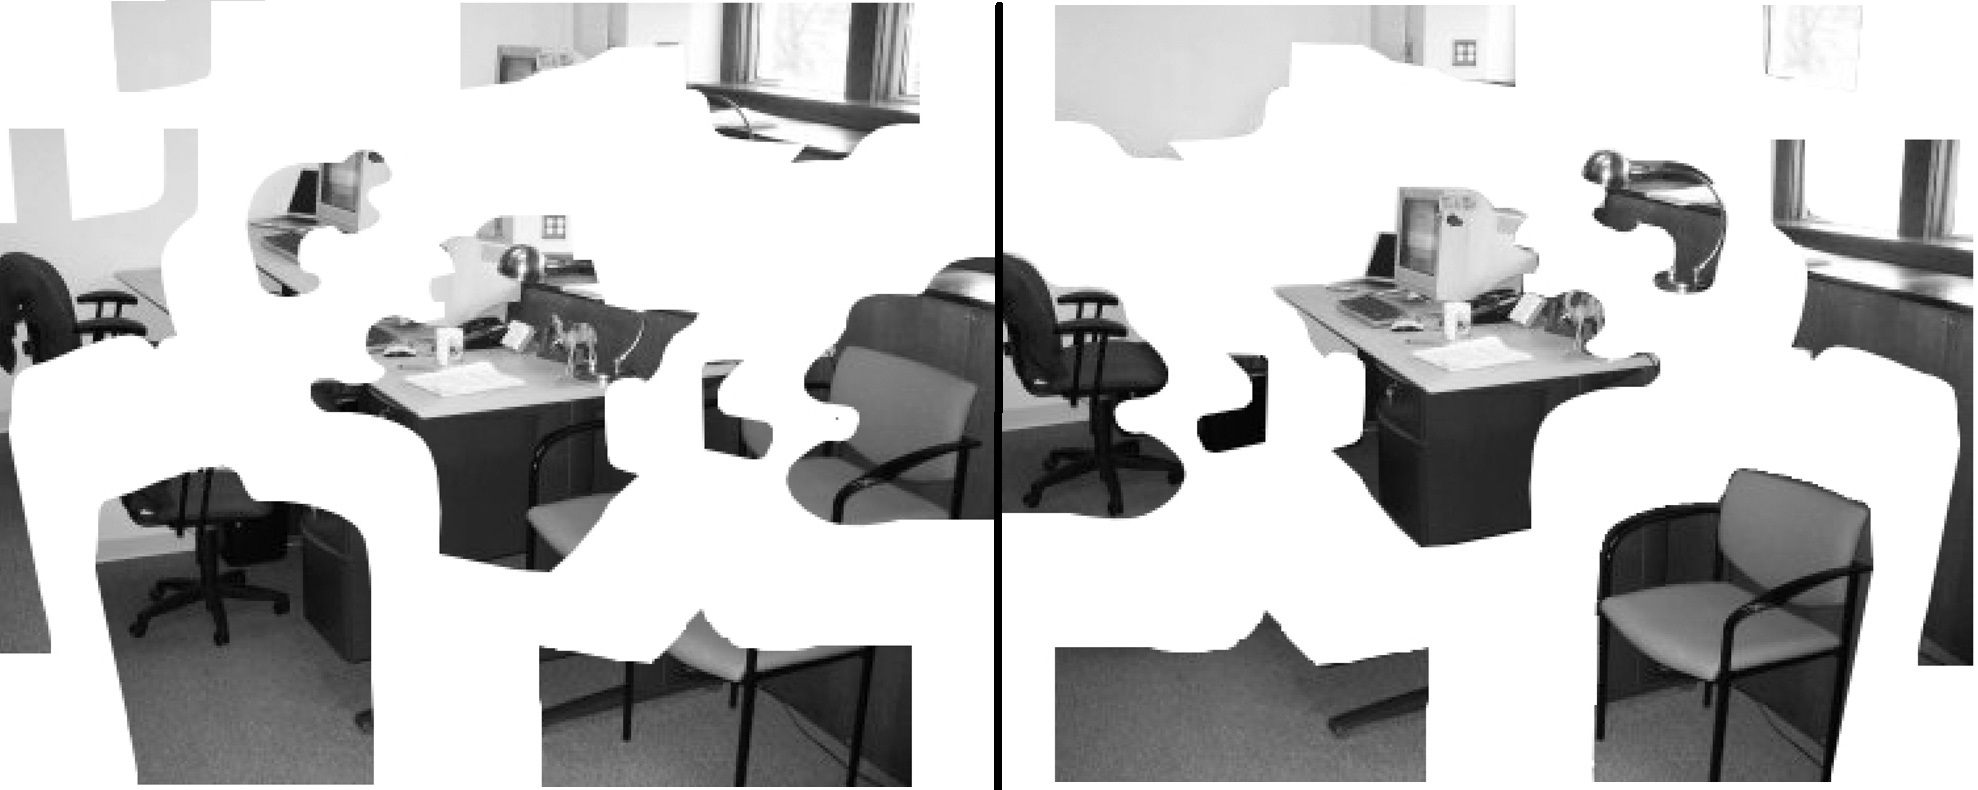
\includegraphics[width=0.9\textwidth, height=130px]{pics/est.jpg}	
	\caption{Ein Bild einer Büroszene in 2 verschiedenen Weisen zerschnitten. Für die linke Version benötigt man mehr Anstrengung um die Szene zu verstehen. Es veranschaulicht, wie eine Zerteilung nach Bedeutung die Wahrnehmung unterstützt. \cite{bib:est}}
	\label{img:est}
\end{figure}
